%%%% ijcai21-multiauthor.tex

\typeout{IJCAI--21 Multiple authors example}

% These are the instructions for authors for IJCAI-21.

\documentclass{article}
\pdfpagewidth=8.5in
\pdfpageheight=11in
% The file ijcai21.sty is NOT the same than previous years'
\usepackage{ijcai21}

% Use the postscript times font!
\usepackage{times}
\renewcommand*\ttdefault{txtt}
\usepackage{soul}
\usepackage{url}
\usepackage[hidelinks]{hyperref}
\usepackage[utf8]{inputenc}
\usepackage[small]{caption}
\usepackage{graphicx}
\usepackage{amsmath}
\usepackage{booktabs}
\urlstyle{same}

%START: added by zhbli
\usepackage{subfigure}  % show sub-figure
\usepackage{algorithm}  % for algrithm
\usepackage{algorithmic}  % for algrithm
\usepackage{multirow}  % for multirow command used in the table
\usepackage{amsfonts}  % for mathbb
\usepackage{color,xcolor}  % 用于改变字体颜色
\usepackage{amssymb}  % 用于打对号
\usepackage{amsfonts}  % 用于 mathbb
%\usepackage{cite}  % 用于引用多篇文献
\newcommand{\eg}{e.g.}
\newcommand{\ie}{i.e.}
%\usepackage{float}  % 如果你确实需要把图片放在当前位置,不容改变,可以用float宏包的[H]选项。
%\usepackage[section]{placeins}  % 如果希望避免浮动体跨过 \section,可以使用 placeins 宏包。
%END: added by zhibi

% the following package is optional:
%\usepackage{latexsym}

% Following comment is from ijcai97-submit.tex:
% The preparation of these files was supported by Schlumberger Palo Alto
% Research, AT\&T Bell Laboratories, and Morgan Kaufmann Publishers.
% Shirley Jowell, of Morgan Kaufmann Publishers, and Peter F.
% Patel-Schneider, of AT\&T Bell Laboratories collaborated on their
% preparation.

% These instructions can be modified and used in other conferences as long
% as credit to the authors and supporting agencies is retained, this notice
% is not changed, and further modification or reuse is not restricted.
% Neither Shirley Jowell nor Peter F. Patel-Schneider can be listed as
% contacts for providing assistance without their prior permission.

% To use for other conferences, change references to files and the
% conference appropriate and use other authors, contacts, publishers, and
% organizations.
% Also change the deadline and address for returning papers and the length and
% page charge instructions.
% Put where the files are available in the appropriate places.

\title{Video-Agnostic Perturbations: Efficient Targeted Attacks \\ for Siamese Visual Tracking}

\iffalse
\author{
Zhenbang Li$^1$\and
Jin Gao$^2$\footnote{Corresponding Author}\and
YaYa Shi$^{2,3}$\and
Bing Li$^4$\and
Pengpeng Liang$^5$\And
Weiming Hu$^6$\\
\affiliations
$^1$First Affiliation\\
$^2$Second Affiliation\\
$^3$Third Affiliation\\
$^4$Fourth Affiliation\\
\emails
\{first, second\}@example.com,
third@other.example.com,
fourth@example.com
}
\else
\author{PaperID: 2266}
\fi

\begin{document}

\maketitle

\begin{abstract}

Siamese trackers are shown to be vulnerable to adversarial attacks recently. However, the existing attack methods craft the perturbations for each video independently, which comes at a non-negligible computational cost. The question is what if we can not get access to the limited computational resources in the real-world online-tracking phase.

In this paper, we show the existence of video-agnostic perturbations that can enable the targeted attack, e.g., forcing a tracker to follow the ground-truth trajectory with specified offsets, to be universal and free from inference in a network. Specifically, we attack a tracker by adding a universal imperceptible perturbation to the template image and pasting a \textit{fake target}, i.e., a small universal adversarial patch, into the search images adhering to the predefined trajectory, so that the tracker outputs the location and size of the \textit{fake target} instead of the real target. Our approach allows perturbing a novel video to come at no additional cost except the mere addition and pasting operations -- and not require gradient optimisation or network inference. Experimental results on several datasets demonstrate that our approach can effectively fool the Siamese trackers in a targeted attack manner. We will make our code publicly available.

\end{abstract}

\section{Introduction}

Given an arbitrary detected or annotated object of interest in the initial video frame, visual object tracking is aimed at {\it recognizing} and {\it localizing} other instances of the same object in subsequent frames. This paradigm of tracking visual objects from a single initial exemplar in the testing phase has been broadly cast as a Siamese network-based one-shot problem recently \cite{SiamFC,SiamRPN,SiamRPN++,SiamFC++}, which is termed as Siamese visual tracking and recognised as highly effective and efficient for visual tracking.

\begin{figure}[htbp]
\centering
%\subfigure{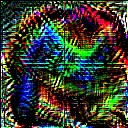
\includegraphics[width=0.2\textwidth]{images/x.jpg}} \qquad
%\subfigure{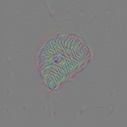
\includegraphics[width=0.2\textwidth]{images/z.jpg}}
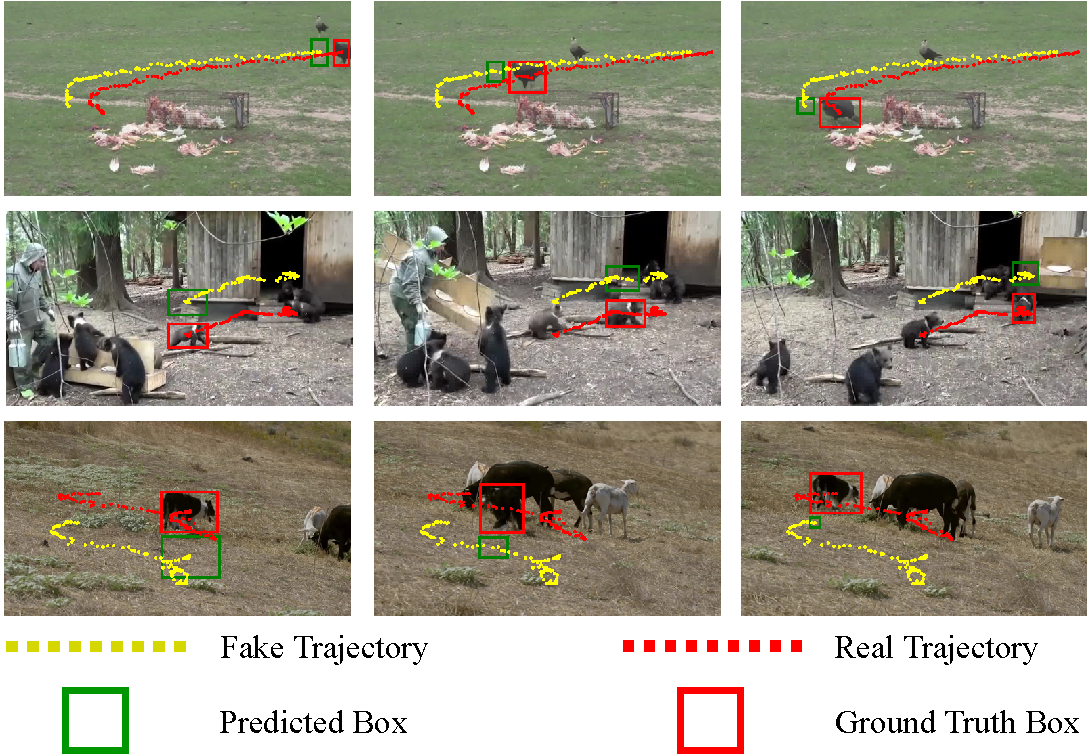
\includegraphics[width=0.48\textwidth]{images/1_v4.pdf}
\caption{Our approach generates the universal perturbations which can be used to attack the Siamese tracker on any video in a targeted manner. Our approach allows perturbing a new video to come at no additional cost except the mere addition and pasting operations -- and not require gradient optimisation or network inference.}
\label{fig:1}
\end{figure}

Recently, the robustness of Siamese trackers have attracted much attention in the sense of testing their vulnerability to adversarial attacks, and the focus has been directed towards more efficient and low-cost attacks \cite{TTP,FAN,SPARK}. Despite their success, these attack methods are not suitable for attacking the real-world online-tracking systems built upon the small edge platforms with limited computational resources. The reason is that they still need to craft the perturbations for each video independently based on either iterative optimisation or adversarial network inference, for which the adequacy of computational resources may be not ensured by the computationally intensive tracking systems. 

Universal adversarial perturbations (UAPs) proposed in \cite{UAP} can fool most images from a data distribution in an image-agnostic manner. Being universal, UAPs can be conveniently exploited to perturb unseen data on-the-fly without extra computations. Therefore, UAPs are particularly useful when attacking real-time applications deployed on platforms with limited computational resources. However, no existing work has touched the topic of attacking the Siamese trackers using UAPs, because it is hard to apply existing UAPs to attack Siamese trackers directly. The main reason lies in the fact that, (a) most UAPs are designed for typical neural networks with one image as input while Siamese networks accept both the template and search images, and (b) the goal of existing UAP methods is to disturb unary and binary model outputs for single instance while we need to use universal perturbations to mislead Siamese trackers to follow a specified trajectory.

In this paper, we make the first attempt in finding the video-agnostic perturbations that fool state-of-the-art Siamese trackers in a targeted attack manner, which comes at virtually no cost in the online-tracking phase. Specifically, we aim to attack the trackers by adding a universal imperceptible perturbation to the template image and pasting a \textit{fake target}, \ie, a small universal adversarial patch, into the search image adhering to the predefined trajectory, so that tracker outputs the location and size of the \textit{fake target} instead of the real target. Our generated video-agnostic perturbations allow perturbing a novel video to come at no additional cost except the mere addition and pasting operations -- and not require gradient optimization or network inference. Experiment results on OTB2015 \cite{OTB}, GOT-10k \cite{GOT-10k} and LaSOT \cite{GOT-10k} datasets demonstrate the effectiveness and efficiency of our approach (see Figure \ref{fig:1}).

\section{Related Work}

\subsection{Siamese Visual Tracking}

Siamese visual tracking is a fundamental research direction in template matching-based tracking besides the correlation filter-based methods. Both of them are aimed to estimate the positions of a template cropped from the initial video frame ``causally" in the subsequent frames. Siamese trackers formulate visual tracking as learning cross-correlation similarities between a target template and the candidates in search region in a convolution fashion. Tracking is then performed by locating the object in the search image region based on the highest visual similarity. This paradigm is formulated as a local one-shot detection task.

Recently, some Siamese trackers~\cite{SiamRPN,SiamRPN++,SiamFC++} have demonstrated a significant performance improvement in visual tracking. 
In particular, SiamRPN \cite{SiamRPN} consists of one Siamese subnetwork for feature extraction and another region proposal subnetwork including the classification and regression branches separately. Based on its success in the decomposition of classification and state estimation, SiamRPN++ \cite{SiamRPN++} further breaks the restriction of strict translation invariance through a simple yet effective spatial aware sampling strategy and successfully trains a ResNet-driven Siamese tracker with significant performance gains. Apart from these anchor-based methods, an anchor-free tracker SiamFC++ \cite{SiamFC++} is further designed by considering non-ambiguous scoring, prior target scale/ratio distribution knowledge-free and estimation quality assessment guidelines.
In our experiments, we are focused on the anchor-free SiamFC++ tracker, whereas the transferability of our generated adversarial attacks to the previous anchor-based trackers is also studied.

\subsection{Adversarial Attacks}

Adversarial attacks to image classification were first investigated in \cite{intriguing}, which is aimed to identify the vulnerability of modern deep networks to imperceptible perturbations. 
Recent studies also emerge to investigate the adversarial attacks to other diverse types of tasks such as natural language processing \cite{generating} and object detection \cite{wei2019transferable}.
Scenarios of possible adversarial attacks can be categorized along different dimensions.

\textit{Imperceptible Perturbations v.s. Adversarial Patch.} The imperceptible perturbations most commonly modify each pixel by a small amount and can be found using a number of optimisation strategies such as Limited-memory BFGS \cite{intriguing} and PGD \cite{PGD}.
Different from the imperceptible perturbations, the adversarial patch is extremely salient to a neural network. The adversarial patch can be placed anywhere into the input image to cause the network to misbehave, and thus is commonly used for universal attacks \cite{patch}.
To the best of our knowledge, we are the first to attack object trackers utilizing both the imperceptible perturbation and the adversarial patch together, which are jointly trained in an end-to-end manner.
Note that our adversarial patch works in the network domain instead of the image domain. In the network-domain case, the noise is allowed to take any value and is not restricted to the dynamic range of images as in the image-domain case \cite{karmon2018lavan}.

\textit{Non-targeted Attacks v.s. Targeted Attacks.} In the case of non-targeted attacks, the adversary's goal is to cause the network to predict any incorrect label and the specific incorrect label does not matter, \eg, pushing the object position estimation just outside the true search region in visual tracking.
Targeted attacks, however, aim to change the network's prediction to some specific target label. In visual tracking, the targeted attacks aim to intentionally drive trackers to output specified object positions following a pre-defined trajectory.

\subsection{Adversarial Attacks in Visual Tracking}

Recently, there are several explorations of the adversarial attacks to the visual tracking task. For example, PAT \cite{PAT} generates physical adversarial textures via white-box attacks to steer the tracker to lock on the texture when a tracked object moves in front of it. However, PAT validates its method by attacking a light deep regression tracker GOTURN \cite{GOTURN}, which has low tracking accuracy on modern benchmarks. In this paper, we aim to attack the state-of-the-art Siamese trackers.
RTAA \cite{RTAA} takes temporal motion into consideration when generating lightweight perturbations over the estimated tracking results frame-by-frame. However, RTAA only performs the non-targeted attacks for trackers, which is less challenging than the targeted attacks in this paper, as we aim to create arbitrary, complex trajectories at test time. 

Targeted attacks to follow an erroneous path which looks realistic are crucial to deceive the tracking system without raising any suspicion in the real-world applications.
SPARK \cite{SPARK} computes incremental perturbations by using information from the past frames to perform targeted attacks to Siamese trackers. However, SPARK needs to generate distinct adversarial example for every search image through heavy iterative schemes, which is time-consuming to attack online-tracking in real time. The recent real-time attacker in \cite{TTP} exclusively uses the template image to generate temporally-transferable perturbations in a one-shot manner, and then adds them to every search image. However, this method still needs to generate perturbations for each individual video, and its targeted attack setting requires diverse perturbations from several runs of network inference. It is ill-suited to attack a real-world online-tracking system when we can not get access to the limited computational resources. In this paper, however, we propose video-agnostic perturbations which allow perturbing a novel video to come at no additional cost except the mere addition and pasting operations.

\begin{figure}[t]
\centering
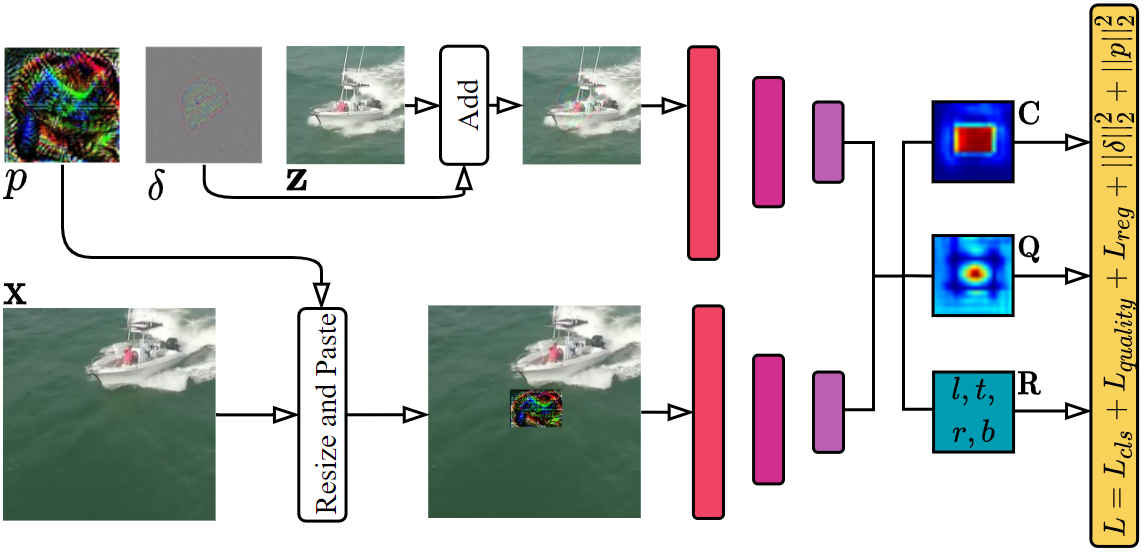
\includegraphics[width=0.48\textwidth]{images/network_v4.png}
\caption{The pipeline of the proposed method. We aim to train an imperceptible perturbation $\delta$ for the template image $\textbf z$, and an adversarial patch $p$ for the search image $\textbf x$. After adding $\delta$ to $\textbf z$ and pasting the fake target $p$ to $\textbf x$, the tracker outputs the location and size of the adversarial patch instead of the real target.}
\label{fig:net}
\end{figure}

\section{Method}

\textcolor{black}{In this section, we introduce our universal targeted attack framework for object trackers based on Siamese networks. We aim to attack the tracker by adding an imperceptible perturbation to the template image and pasting a \textit{fake target}, i.e., an adversarial patch into the search image adhering to the predefined trajectory, so that the tracker outputs the location and size of the fake target instead of the real target. Below, we formalize the task of performing universal targeted attacks on an object tracker, and then introduce our perturbation strategy in detail.}
 
\subsection{Problem Definition}

Let $V=\{I_i\}_1^T$ denote the frames of a video sequence of length $T$.
$B^{gt}=\{b^{gt}_i\}_1^T$ is used to represent the target's ground-truth position in each frame.
The visual object tracking will predict the position $B^{pred}=\{b^{pred}_i\}_1^T$ of this target in the subsequent frames when given its initial state.
In SiamFC++ \cite{SiamFC++}, the tracker first transforms the reference frame $I_1$ and annotation $b_1^{gt}$ to get an template image $\textbf z$, and transforms the candidate frame $I_i$ to get the search image $\textbf x_i$ centered at the position obtained in the previous frame.
At each time-step, the template image $\textbf z$ and the search image $\textbf x_i$ are first passed individually through a shared backbone network, and the resulting features are processed by some non-shared layers and fused by depth-wise separable correlation. The fused features then act as input to a head network, which predicts a classification map $\textbf{C}$, a bounding box regression map $\textbf{R}$, and a quality assessment map $\textbf{Q}$. In short, $\textbf C$ encodes the probability of each spatial position to contain the target, $\textbf R$ regresses the bounding box position of the target, and $\textbf Q$ predicts the target state estimation quality. The final bounding box is then generated according to $\textbf{C}$, $\textbf{R}$ and $\textbf{Q}$.

Formally, we aim to train an imperceptible perturbation $\delta$ for the template image $\textbf z$, and an adversarial patch $p$ for the search image $\textbf x$. After adding $\delta$ to $\textbf z$ and pasting the fake target $p$ to $\textbf x$, the tracker outputs the location and size of the adversarial patch instead of the real target (see Figure \ref{fig:net}).
Both $\delta$ and $p$ are universal (i.e., video-agnostic), which means perturbing a new video only involves the mere addition/paste of the perturbations to the template/search image -- and does not require gradient optimisation or network inference.

\begin{algorithm}[tb]
\caption{Training Process}
\label{alg:algorithm}
\textbf{Input}: Training dataset $\mathcal{V}$, Siamese tracker $\phi$, and max iteration number $N$.\\
\textbf{Output}: Universal perturbation $\delta$, and universal patch $p$.
\begin{algorithmic}[1] %[1] enables line numbers
\STATE Let $k = 0$.
\WHILE{$k < N$}
\STATE Randomly pick a video $V\in \mathcal{V}$. The corresponding ground truth is $B^{gt}=\{b^{gt}_i\}^T_1$.
\STATE Randomly pick two frames $I_t, I_s$ from $V$.
\STATE Generate template image $\textbf{z}$ according to $I_t$ and $b^{gt}_t$.
\STATE $\tilde{\textbf{z}} = \textbf{z} + \delta_k.$
\STATE Generate search image $\textbf{x}$ according to $I_s$ and $b^{gt}_s$.
\STATE Calculate the fake target position $\{l^x, l^y, w, h\}$ relative to the search image.
\STATE $\tilde{\textbf x} = A(\textbf x, p_k, (l^x, l^y), (w, h)).$
\STATE $\textbf{C, R, Q} = \phi(\tilde {\textbf x}, \tilde{\textbf z}).$
\STATE Generate fake labels $\textbf{C}^*,\textbf{R}^*,\textbf{Q}^*$ using $\{l^x, l^y, w, h\}$.
\STATE Calculate loss $L(\textbf{C, R, Q}, \textbf{C}^*, \textbf{R}^*, \textbf{Q}^*)$ using Equ. \ref{eq:loss}.
\STATE $\delta_{k+1} = \delta_{k} - \epsilon_1 \cdot \text{sign}(\nabla_{\delta_k}L).$
\STATE $p_{k+1} = p_{k} - \epsilon_2 \cdot \text{sign}(\nabla_{p_k}L).$
\STATE $i = i + 1.$
\ENDWHILE
\STATE \textbf{return} $\delta_N, p_N.$
\end{algorithmic}
\end{algorithm}

\begin{figure*}[t]
\centering
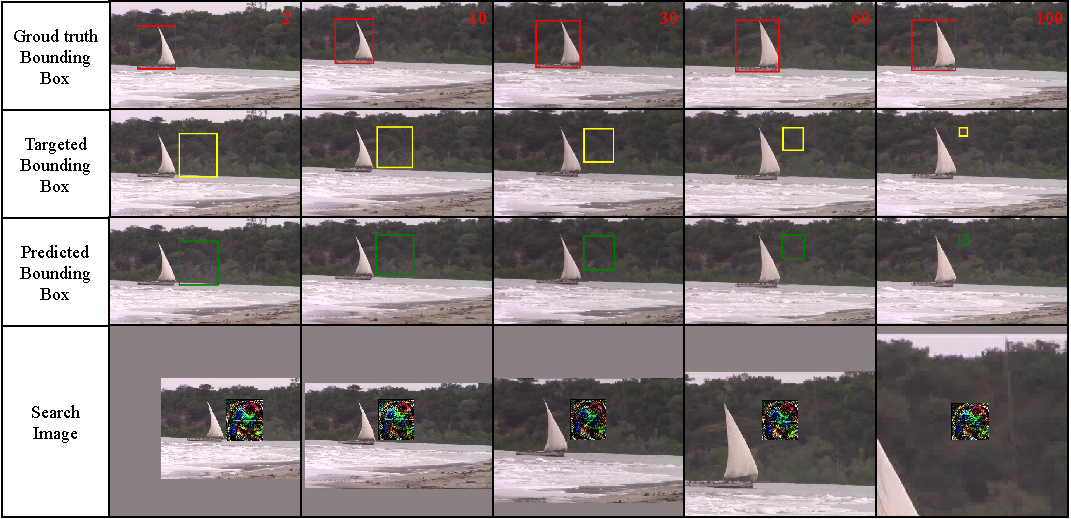
\includegraphics[width=0.80\textwidth]{images/vis_v3.pdf}
\caption{The results under targeted attacks. Red represents a ground-truth bounding box, yellow represents the specific bounding box, and green represents the predicted bounding box by trackers. The yellow and green boxes are basically the same in time series, which indicates that the targeted attack is successful.}
\label{fig:vis}
\end{figure*}

\subsection{Generating Universal Perturbations}

In this subsection, we show how to train the universal perturbations $(\delta, p)$ for Siamese trackers (see Algorithm 1).
During the $k$-th iteration of training, a video $V=\{I_i\}_1^T$ is randomly selected from the training dataset $\mathcal V$. Assuming the template perturbation at the $k$-th iteration is $\delta_k \in \mathbb{R}^{127\times 127 \times 3}$, and the adversarial patch is $p_k \in \mathbb{R}^{128\times 128\times 3}$. We first randomly pick two frames $I_t, I_s$ from $V$.
The clean template image $\textbf z\in \mathbb{R}^{127\times 127 \times 3}$ is generated according to $I_t$ and $b^{gt}_t$, and the perturbed template image is:
\begin{equation}
\tilde {\textbf z} = \textbf z + \delta_i.
\end{equation}
Similarly, the clean search image $\textbf x \in \mathbb{R}^{303\times 303 \times 3}$ is generated according to $I_s$ and $b^{gt}_s$.
As mentioned before, the patch is regarded as a fake target and pasted on the search image. We force the center position of the fake target to near the center position of the real target (i.e., the center of the search image) with a shift range of 64 pixels, where shift is defined as the max range of translation generated by a uniform distribution.
The width/height of the fake target is randomly selected between 32 pixels and 128 pixels.
The perturbed search image is generated as follows:
\begin{equation}
\tilde{\textbf x} = A(\textbf x, p_k, (l^x, l^y), (w, h)),
\end{equation}
where $(l^x, l^y)$ and $(w, h)$ represents the position and size of the fake target relative to the search image, respectively. $A$ is \textit{patch application operator} \cite{patch} which first resizes the patch $p_k \in \mathbb{R}^{128\times 128\times 3}$ to $\hat{p}_k \in \mathbb{R}^{w\times h\times 3}$, and then applies the resized patch $\hat{p}_k$ to the search image $\textbf x$ at location $(l^x,l^y)$.

Subsequently, the SiamFC++ tracker $\phi(\cdot)$ takes $\tilde {\textbf x}$ and $\tilde{\textbf  z}$ as input and makes predictions as follows:
\begin{equation}
\textbf{C, R, Q} = \phi(\tilde {\textbf x}, \tilde{\textbf z}),
\end{equation}

\subsubsection{Training Objective}

The loss function is calculated as follows:
\begin{equation}
\begin{array}{l}
\begin{aligned}
L&=\frac{\alpha}{N_{\mathrm{pos}}} \sum_{x, y} L_{\mathrm{cls}}\left(\textbf{C}_{x, y}, \textbf{C}_{x, y}^{*}\right) \\
&+\frac{\beta}{N_{\mathrm{pos}}} \sum_{x, y} \textbf{1}_{\left\{\textbf{C}_{x, y}^{*}>0\right\}} L_{\mathrm{quality}}\left(\textbf{Q}_{x, y}, \textbf{Q}_{x, y}^{*}\right) \\
&+\frac{\gamma}{N_{\mathrm{pos}}} \sum_{x, y} \textbf{1}_{\left\{\textbf{C}_{x, y}^{*}>0\right\}} L_{\mathrm{reg}}\left(\textbf{R}_{x, y}, \textbf{R}_{x, y}^{*}\right) \\
&+\eta \cdot ||\delta_k||_2^2 +  \sigma \cdot ||p_k||^2_2,
\end{aligned}
\end{array}
\label{eq:loss}
\end{equation}
\textcolor{black} %(SiamFC++)
{where $\textbf{C}_{x, y}, \textbf{R}_{x, y}, \textbf{Q}_{x, y}$ represent the values of $\textbf{C}, \textbf{R}, \textbf{Q}$ at location $(x, y)$, respectively. $\textbf{C}^*, \textbf{R}^*, \textbf{Q}^*$ are the fake labels generated according to the position/size of the fake target.$\textbf 1$ is the indicator function that takes 1 if the condition in subscribe holds and takes 0 if not, $L_{\mathrm{cls}}$ denote the focal loss for classification result, $L_{\mathrm{quality}}$ denote the binary cross entropy (BCE) loss for quality assessment and $L_{\mathrm{reg}}$ denote the IoU loss \cite{iou-loss} for bounding box result. Following SiamFC++, we assign 1 to $\textbf{C}_{x, y}^{*}$ if $(x, y)$ is considered as a positive sample, and 0 if as a negative sample.}

\begin{table*}
\centering
\scriptsize
\tabcolsep=4.0pt
%\resizebox{\textwidth}{!}{%
\label{tab:iter}
\begin{tabular}{cc|cccccccccccccccc} 
\toprule
\multicolumn{2}{c|}{Iterations}     & 1     & 2     & 4     & 8     & 16    & 32    & 64    & 128   & 256   & 512   & 1024  & 2048  & 4096  & 8192  & 16384 & 32768  \\ 
\midrule
\multirow{2}{*}{Fake Trajectory} & AO    & 0.002 & 0.002 & 0.002 & 0.002 & 0.002 & 0.003 & 0.007 & 0.042 & 0.299 & 0.668 & 0.746 & 0.781 & 0.798 & 0.820 & 0.821 & 0.818  \\
                                 & SR    & 0.000 & 0.000 & 0.000 & 0.000 & 0.000 & 0.001 & 0.005 & 0.044 & 0.335 & 0.749 & 0.822 & 0.855 & 0.872 & 0.895 & 0.897 & 0.890  \\ 
\midrule
\multirow{2}{*}{Real Trajectory} & AO    & 0.757 & 0.756 & 0.757 & 0.757 & 0.758 & 0.759 & 0.753 & 0.720 & 0.474 & 0.150 & 0.095 & 0.071 & 0.041 & 0.032 & 0.032 & 0.035  \\
                                 & SR    & 0.894 & 0.891 & 0.893 & 0.891 & 0.893 & 0.896 & 0.888 & 0.852 & 0.559 & 0.164 & 0.098 & 0.066 & 0.031 & 0.021 & 0.022 & 0.023  \\ 
\midrule
\multicolumn{2}{c|}{SSIM of $\delta$}                        & 1.00  & 1.00  & 1.00  & 1.00  & 0.99  & 0.99  & 0.97  & 0.93  & 0.86  & 0.86  & 0.87  & 0.88  & 0.88  & 0.88  & 0.88  & 0.88   \\
%\multicolumn{2}{c|}{MSE}                         & 0.51  & 0.26  & 0.32  & 0.37  & 0.48  & 0.84  & 2.03  & 5.65  & 15.10 & 25.43 & 23.70 & 21.89 & 20.69 & 20.49 & 20.03 & 20.87  \\
\bottomrule
\end{tabular}
%}
\caption{Influence of the number of training iterations on GOT-10k\_Val.}
\label{tab:iter}
\end{table*}

\subsubsection{Optimisation}

At each training step, the perturbations are updated as follows:
\begin{gather}
\delta_{k+1} = \delta_{k} - \epsilon_1 \cdot \text{sign}(\nabla_{\delta_k}L)\\
p_{k+1} = p_{k} - \epsilon_2 \cdot \text{sign}(\nabla_{p_k}L),
\end{gather}
where $\epsilon_1$ is used to ensure that the perturbation added to the template image is imperceptible, and $\epsilon_2$ is used to maintain the training stability.
During training, we only optimize the values of perturbations $(\delta, p)$, and the parameters of the Siamese network remain intact.

\begin{table}[thbp]
\centering
\scriptsize
\tabcolsep=2.0pt
%\resizebox{0.48\textwidth}{!}{%
\begin{tabular}{c c | c | c | c}
\toprule
\multirow{2}{*}[-2pt]{Trackers} & \multirow{2}{*}[-2pt]{Metric} & Clean Videos    & \multicolumn{2}{c}{Perturbed Videos}  \\
\cmidrule{3-5}
                          &                         & Real Trajectory & Real Trajectory & Fake Trajectory     \\ 
\midrule
\multirow{2}{*}{OTB-15} 
& Success   & 0.642 & 0.035 & 0.842\\
& Precision & 0.861 & 0.048 & 0.928\\
\midrule
\multirow{3}{*}{GOT-Val} 
& SR & 0.897 & 0.023 & 0.890\\
& AO 				   & 0.760 & 0.035 & 0.818 \\
\midrule
\multirow{4}{*}{LaSOT} 
& Prec.       & 0.514 & 0.013 & 0.820\\
& Norm. Prec. & 0.551 & 0.015 & 0.788\\
& Succ. Score & 0.525 & 0.022 & 0.767\\
& Succ. Rate  & 0.626 & 0.016 & 0.834\\
\midrule
\multicolumn{2}{c|}{FPS} & 58 & 58 & 58\\
\bottomrule
\end{tabular}
%}
\caption{Attack results on several benchmarks.}
\label{tab:benchmark results}
\end{table}

\subsection{Attacking the Tracker at Inference Time}

Once the perturbations $(\delta, p)$ is trained, we can use them to perturb the template image and search images of any natural video. Both $\delta$ and $p$ are universal (i.e., video-agnostic), which means perturbing a new video only involves the mere addition/paste of the perturbations to the template/search image -- and does not require gradient optimisation or network inference.
Assume $B^{fake}=\{b^{fake}_i\}_1^{T}$ is the trajectory we hope the tracker to output.
During tracking the $i$-th frame of the video $V=\{I_i\}_1^T$, we need to transform the bounding box $b^{fake}_i$ (relative to the original frame $I_i$) into the box $\hat b_i=\{l^x_i, l^y_i, w_i, h_i\}$ relative to the search image $\textbf x_i$, and paste $p$ into $\textbf x_i$ according to $\hat b_i$:
\begin{equation}
\tilde{\textbf x}_i = A(\textbf x_i, p, (l^x_i, l^y_i), (w_i, h_i)).
\end{equation}
The tracker then takes $\tilde{\textbf z}_i=\textbf z_i+\delta$ and $\tilde{ \textbf x}_i$ as input, and the subsequent tracking procedure remains the same as SiamFC++.

%%%%%%%%%%%%%%%%%%%%%%%%%%%%%%%%%%%%%%%%%%%%%%%%%%%%%%%%%%%%
%%%%%%%%%%%%%%%%%%%%%%%%%%%%%%%%%%%%%%%%%%%%%%%%%%%%%%%%%%%%
\section{Experiments}

\subsection{Setting}

\subsubsection{Implementation Details}

We use SiamFC++ \cite{SiamFC++} as our base tracker, and the backbone Siamese network adopts GoogLeNet \cite{GoogLeNet}.
We implement our approach in Pytorch and train our perturbations using 3 GTX 1080Ti GPUs.
We adopt GOT-10k \cite{GOT-10k}, COCO \cite{COCO}, ILSVRC-VID \cite{VID} and LaSOT \cite{LaSOT} and our training set.
We train the perturbations for 32768 iterations with a minibatch of 96 images (32 images per GPU).
The learning rate of the template perturbation $\epsilon_1$ is set to 0.1, and the learning rate of the adversarial patch is $\epsilon_2 = 0.5$.
We generate training samples following the strategy in SiamFC++.
During the training and the testing phase, the size of the template image is set to $127\times 127\times 3$, and the size of the search image is set to $303\times 303\times 3$.
In Equ. \ref{eq:loss}, we set $\alpha=1, \beta=1, \gamma=1, \eta=0.005, \sigma=10^{-5}$.

\subsubsection{Datasets}
We evaluate our universal perturbations on several tracking datasets: OTB2015 \cite{OTB}, GOT-10k\_Val \cite{GOT-10k}, and LaSOT \cite{LaSOT}.
The detailed information and evaluation metrics of each dataset are described in the following subsections.

\subsubsection{Generating the Fake Trajectory}

We need to set a specific trajectories $B^{fake}=\{b^{fake}_i\}_1^{T}$ for each video in the dataset to achieve targeted attack, which we call the \textit{fake trajectory}. We call the bounding box ground truth $B^{gt}=\{b^{gt}_i\}_1^T$ the \textit{real trajectory}.
Manually labelling $B^{fake}$ for each video will be time-consuming, so we generate $B^{fake}$ based on $B^{gt}$.
Specifically, the fake trajectory follows the real trajectory and the boundary between $b^{fake}_i$ and $b^{gt}_i$ is 16 pixels apart.
%The size of $b^{fake}_0$ is the same as $B^{gt}_0$ and the size of $b^{fake}_i$
The bounding box size of the fake trajectory gradually changes from the size of $b^{gt}_1$ to $64\times 64$.

\subsubsection{Image Quality Assessment} We use structural similarity (SSIM) to evaluate the quality of the template perturbation $\delta$. The generated adversarial perturbation is difficult to be found when SSIM is close to 1 (see Table \ref{tab:iter}).

\subsection{Result on Several Benchmarks}

We test the performance of our attack method on several benchmarks and results are gathered in Table \ref{tab:benchmark results}.
%Note that, in the original SiamFC++ paper, they test different dataset using different trained model. But we test them using one single model. So on some datasets will drop slightly.

\begin{table}[t]
\centering
\scriptsize
\tabcolsep=2.0pt
%\resizebox{0.48\textwidth}{!}{%
\begin{tabular}{ccc|cc|cc} 
\toprule
\multirow{2}{*}[-2pt]{$L_{\text{cls}}$}     & \multirow{2}{*}[-2pt]{$L_{\text{quality}}$} & \multirow{2}{*}[-2pt]{$L_{\text{reg}}$} & \multicolumn{2}{c|}{Fake Trajectory}          & \multicolumn{2}{c}{Real Trajectory}           \\ 
\cmidrule{4-7}
                       &                    &                    & AO                    & SR                    & AO                    & SR                     \\ 
\midrule
\checkmark   &    &    & 0.718  & 0.824    & 0.086 & 0.083   \\
   & \checkmark   &    & 0.044  & 0.044    & 0.703 & 0.842   \\
   &    & \checkmark   & 0.664  & 0.726    & 0.165 & 0.184   \\
\checkmark   & \checkmark   & \checkmark   & 0.781  & 0.855    & 0.071 & 0.066   \\ \bottomrule
\end{tabular}
%}
\caption{Contribution of each loss on GOT-10k\_Val.}
\label{tab:loss}
\end{table}

\subsubsection{Evaluation on OTB2015 Benchmark}

As one of the most classical benchmarks for the object tracking task, the OTB benchmark provides a fair test for trackers. We conduct experiments on OTB2015 \cite{OTB} which contains 100 videos for tracker performance evaluation.
We use success precision and success scores to evaluate the performance of trackers on the OTB2015 dataset.
The precision encodes the proportion of frames for which the center of the tracking window is within 20 pixels of the ground-truth center. The success corresponds to the proportion of frames for which the overlap between the predicted and ground truth tracking window is greater than a given threshold.
After applying the universal perturbations to videos, the success score relative to $B^{gt}$ drops from 0.642 to 0.035, indicating that our method can fool the state-of-the-art SiamFC++ tracker on OTB2015 effectively.
%The success score relative to $B^{gt}$ on the clean videos is 0.642. The success score relative to $B^{gt}$ on the adversarial videos is 0.035. The success score relative to $B^{fake}$ on the adversarial videos is 0.842.

\subsubsection{Evaluation on GOT-10k Benchmark}

GOT-10k \cite{GOT-10k} is a recent large-scale high-diversity dataset. There is no overlap in object classes between the train/val/test splits, promoting the importance of generalization to unseen object classes.
%Because we need to use the real ground truth to generate the fake ground truth, and the fake ground truth is not available on test set, so we use the val set.
%The evaluation metric is AO and Success rate, which means ...
We use the average overlap (AO) for evaluation.
The AO relative to $B^{fake}$ on the adversarial videos is 0.818, which demonstrates that the generated universal perturbations can mislead the track to follow a specified trajectory (see Figure \ref{fig:vis}).

\subsubsection{Evaluation on LaSOT Benchmark}

With a large number of video sequences, LaSOT (Largescale Single Object Tracking) benchmark \cite{LaSOT} makes it impossible for trackers to overfit the benchmark, which achieves the purpose of testing the real performance of object tracking.
Following onepass evaluation, we use three criteria including precision, normalized precision and success for evaluation.
The precision score relative to $B^{gt}$ on the clean videos is 0.514. The precision score relative to $B^{gt}$ on the adversarial videos is 0.013. The precision score relative to $B^{fake}$ on the adversarial videos is 0.820, indicating that our attack method is effective. Being universal, the generated perturbations can be conveniently exploited to perturb videos on-the-fly without extra computations.

\subsubsection{Compared with Other Methods}

In Table \ref{tab:untargeted}, we compare the untargeted attack performance of our method with CSA \cite{CSA}, FAN \cite{FAN} and TTP \cite{TTP}.
We report the precision score relative to the real trajectory on OTB2015.
Our method significantly outperforms other methods in terms of the drop rate of the precision score.

In Table \ref{tab:targeted}, we compare the targeted attck performance of our method with FAN \cite{FAN} and TTP \cite{TTP}.
Our method significantly outperforms other methods in terms of the precision score relative to the fake trajectory on OTB2015.

\begin{table}[t]
\centering
\scriptsize
\tabcolsep=2.0pt
%\resizebox{\textwidth}{!}{%
\begin{tabular}{@{}ccc|cccc@{}}
\toprule
Method & Tracker & Backbone & \begin{tabular}[c]{@{}c@{}}Attack\\ Cost(ms)\end{tabular} & \begin{tabular}[c]{@{}c@{}}Clean\\ Videos\end{tabular} & \begin{tabular}[c]{@{}c@{}}Perturbed\\ Videos\end{tabular} & \begin{tabular}[c]{@{}c@{}}Drop\\ Rate\end{tabular} \\ \midrule
CSA & SiamRPN & AlexNet & 4720 & 0.851 & 0.458 & 0.46 \\
FAN & SiamFC & AlexNet & 10 & 0.720 & 0.180 & 0.75 \\
TTP & SiamRPN++ & ResNet-50 & 8 & 0.910 & 0.080 & 0.91 \\
\midrule
Ours & SiamFC++ & GoogLeNet & 0 & 0.861 & 0.048 & 0.94 \\ \bottomrule
\end{tabular}%
%}
\caption{Precision score relative to the real trajectory on OTB2015.}
\label{tab:untargeted}
\end{table}

\begin{table}[t]
\centering
\scriptsize
\tabcolsep=2.0pt
%\resizebox{0.48\textwidth}{!}{%
\begin{tabular}{@{}cccc@{}}
\toprule
Method & Tracker & Backbone & \begin{tabular}[c]{@{}c@{}}Precision on\\ Perturbed Videos\end{tabular}  \\ \midrule
FAN & SiamFC & AlexNet & 0.420 \\
TTP & SiamRPN++ & ResNet-50 & 0.692 \\
\midrule
Ours & SiamFC++ & GoogLeNet & 0.928 \\
\bottomrule
\end{tabular}%
%}
\caption{Precision score relative to the fake trajectory on OTB2015.}
\label{tab:targeted}
\end{table}

\subsection{Ablation Studies}

\subsubsection{Influence of Training Loss}

We implement a series of experiments to analyse and evaluate the contribution of each loss component.
In Table \ref{tab:loss}, we report our results on GOT-10k val set with different combination of loss terms, where $L_{\text{cls}}, L_{\text{quality}}, L_{\text{reg}}$ represent the classification loss, the quality assessment loss and the regression loss in Equ. \ref{eq:loss}, respectively.
To summarize, while all loss terms are beneficial, the classification term is more efficient than the quality assessment term. 

\subsubsection{Influence of Training Iterations}

As shown in Table \ref{tab:iter}, after approximately 30000 training iterations, the generated perturbations could fool most targets in GOT-10k\_Val. The AO relative to $B^{gt}$ falls down from 0.760 to 0.035. We notice that at the start of the training period (when training iteration is less than 2048), the falling speed of AO relative to $B^{gt}$ is the largest. This demonstrates the efficiency of our end-to-end training pipeline used to generate the adversarial perturbations.

\subsection{Transferability}

\subsubsection{Transferability of Different Backbones}

We evaluate the transferability of our attacks on different backbones of SiamFC++: ShuffleNet \cite{ShuffleNet} and AlexNet \cite{AlexNet}.
The experimental results are shown in Table \ref{tab:backbone}. On SiamFC++-AlexNet, the AO relative to $B^{gt}$ drops from 0.72 to 0.196. However, our perturbations do not generalize well on SiamFC++-ShuffleNet, which we conjecture to be due to the significant difference of the network structure between GoogLeNet and ShuffleNet.

\begin{table}[t]
\begin{center}
\scriptsize
\tabcolsep=2.0pt
%\resizebox{0.48\textwidth}{!}{%
\begin{tabular}{c|cc|cc|cc} 
\toprule
\multirow{3}{*}[-6pt]{Backbone} & \multicolumn{2}{c|}{Clean Videos}    & \multicolumn{4}{c}{Perturbed Videos}                                        \\ 
\cmidrule{2-7}
                          & \multicolumn{2}{c|}{Real Trajectory} & \multicolumn{2}{c|}{Real Trajectory} & \multicolumn{2}{c}{Fake Trajectory}  \\ 
\cmidrule{2-7}
                          & AO    & SR                           & AO    & SR                           & AO    & SR                           \\ 
\midrule
GoogLeNet                 & 0.760 & 0.897                        & 0.035 & 0.023                        & 0.818 & 0.890                        \\
AlexNet                   & 0.720 & 0.850                        & 0.196 & 0.227                        & 0.572 & 0.640                        \\
ShuffleNet                & 0.766 & 0.888                        & 0.554 & 0.656                        & 0.135 & 0.134                        \\
\bottomrule
\end{tabular}
%}
\end{center}
\caption{Transferability of different backbones on GOT-10k\_Val.}
\label{tab:backbone}
\end{table}

\subsubsection{Transferability of Different Tracking Architectures}

We use AlexNet-based SiamRPN \cite{SiamRPN} and ResNet-based SiamRPN++ \cite{SiamRPN++} as black-box attack models to verify the transferability of our perturbations on different tracking architectures.
SiamRPN uses an RPN network to perform location regression and classification on the response map. SiamRPN++ performs layer-wise and depth-wise aggregation to improve accuracy. Both SiamRPN and SiamRPN++ are anchor-based methods while SiamFC++ is an anchor-free method.
The experimental results are shown in Table \ref{tab:arch}. On SiamRPN, the success score relative to $B^{gt}$ drops from 0.666 to 0.379. On SiamRPN++, the success score relative to $B^{gt}$ drops from 0.676 to 0.518. The results show that our method can still show good transferability for different tracking architectures.

\begin{table}[t]
\centering
\scriptsize
\tabcolsep=2.0pt
%\resizebox{0.48\textwidth}{!}
\caption{Transferability of different tracking architectures on OTB2015.}
\label{tab:arch}
\end{table}

\section{Conclusion}

In this paper, we propose a universal targeted attack method for Siamese trackers. 
We aim to attack the tracker by adding an imperceptible perturbation to the template image and pasting a \textit{fake target}, i.e., a small adversarial patch into the search image adhering to the predefined trajectory, so that tracker outputs the location and size of the fake target instead of the real target. An end-to-end pipeline is proposed to train the perturbations efficiently.
Experiments on several popular datasets show that our method can effectively fool the Siamese trackers in a targeted attack manner.

\clearpage
\bibliographystyle{named}
\bibliography{ijcai21}

\iffalse
\section{Useless Sentences}

\subsection{How we set identify the fake path ?}

There are several methods to control the box direction. One is to generate several pre-trained perturbations, one represents a specific direction. During testing, a best direction is selected according to the fake GT position. However, there are some disadvantages of this method:
\begin{itemize}
\item They need several pre-trained perturbations. If they want more accurate, they need more pre-train.
\item They generate the approximate trajectory.
\item They have to generate  new perturbations of A new video.
\end{itemize}
To overcome these disadvantages, we use a small patch to control the prediction. So we can make the network to predict any shape/position as what we want. And we are universal.

our loss function is:
\begin{equation}
L = \alpha \cdot L_{cls} + \beta \cdot L_{ctr} +  \gamma \cdot L_{reg} + \eta \cdot ||z||_2^2 +  \sigma \cdot ||x||^2_2
\end{equation}

We will generate the fake ground truth $GT^{\text{fake}}=\{B^{fake}_i\}_1^T$.
We will predict: $\{B^{pred}_i\}_1^T$.
The tracker is $\phi$, we get the prediction $B_i^{pred}=\phi(z, x_i)$.

$z = \tau (I_1, b^{gt}_1)\in \mathcal{R}^{127\times 127\times 3}$

$x = \tau(I_i, b_{i-1}^{pred})\in \mathcal{R}^{303\times 303 \times 3}$

at each spatial location, the classification map encodes the probability of each position to contain the target, the regression map produces a corresponding offset, and the quality assessment map give the quality. 

which predicts a classification map $\textbf{C}\in \mathbb{R}^{H\times W\times 1}$, a bounding box regression map $\textbf{R}\in \mathbb{R}^{H\times W\times 4}$, and a quality assessment map $\textbf{Q}\in \mathbb{R}^{H\times W\times 1}$.

We want them universal so that no extra time is needed.
For targeted attack, suppose a fake trajectory $GT^{\text{fake}}=\{B^{fake}_i\}_1^T$ is what we hope the tracker to output, we want to drive trackers to output desired object positions specified by the targeted trajectory. This is achieved by the patch position: We paste the patch to the specified position, and we hope the tracker prediction to the patch position (i.e., the FGT).

Then we generate the perturbed template image and search image, then we generate the fake label, then we make prediction, calculate loss, and update perturbations for one iteration.

$z = \tau (I_j, b^{gt}_j)\in \mathcal{R}^{127\times 127\times 3}$

Note that we control the $\delta$ to be small. The shape of $\delta$ is $127 \times 127 \times 3$, and the shape of the $z$ is also $127 \times 127 \times 3$.

First we generate the clean search image is cropped at the center of the target:$x = \tau(I_k, b_{k}^{gt})\in \mathcal{R}^{303\times 303 \times 3}$

Then we set up the fake box in the search image. The center position of our patch is randomly put [-64, 64] near to the real target. The size of our patch is randomly from [-32, 128], to model the different size/position of the target. So we get the fake box $\hat b$. Note that $\hat b$ is relevant to the search image.

\subsubsection{Generating the Fake Label}

According to SiamFC++, there are three labels: classification label, regression label and quality assessment label.
We generate fake ground truth $\hat y$ according to patch shape/position on the search image  used for calculate loss.
We use the position of this fake GT to generate the $\hat y$.
We need the network prediction close to the FGT.
Calculate the FGT box position on the search image, according to the scale.
We generate the fake label of the tracker according to the position of the fake target:
\begin{equation}
\mathcal{C^*, Q^*, T^*} = A(m),
\end{equation}
where classification GT $S_{cls} \in R^{19 \times 19 \times 1}$, where $S_{cls}(x,y)$ denotes the classification confidence score for the box at spatial position $(x,y)$. The center GT $S_{ctr} \in \mathbb{R}^{19 \times 19 \times 1}$, where $S_{ctr}(x,y)$ denotes the quality assessment score for box at $(x,y)$, and regression GT $S_{reg} \in \mathbb{R}^{19 \times 19 \times 4}$, where $S_{reg}(x,y) \in \mathbb R^{4}$ is the delta of $B^{fake}$.

and the fake label $\tilde y$

where $y$ includes three parts: classification map $CLS \in R^{19 \times 19 \times 1}$, regression map $REG \in \mathbb{R}^{19 \times 19 \times 1}$, and center map $CTR \in \mathbb{R}^{19 \times 19 \times 4}$.

\subsubsection{Loss Function}

We use the trained network of SiamFC++ \cite{SiamFC++}.
It is an anchor free method for tracking. It contains three losses to train the tracker: classification loss, center loss and regression loss.

\subsection{Abstract}

In this paper, we propose a new method to attack the Siamese trackers. 
We \textbf{first} propose the \textbf{universal} attack for Siamese trackers, we achieve it by use the small distribution on the template image and use the patch on the search image.
We use a \textbf{fake target}, i.e., a small patch onto the search image, to guide the tracker to prediction badly.
We not only to attack by the fake target, we also manipulate the template image to boost the performance.
Different from the existing tracker attack method, we can not only control the trajectory of the target, but also the size of the target.
Our code is public at https://github.com/lizhenbang56/Universal-Targeted-Attacks-for-Siamese-Visual-Tracking
\textit{(D PATCH) Unlike the original adversarial patch that only manipulates image-level classifier, our patch simultaneously attacks the bounding box regression and object classification so as to disable their predictions.}
We propose a systematic algorithm for computing universal perturbations, and show that state-of-the-art Siamese trackers are highly vulnerable to such perturbations.

In SiamFC++, the tracker $\phi(\cdot)$ first transforms the reference frame $I_1$ and annotation $b_1$ to get an template image $z = \tau (I_1, b^{gt}_1)\in \mathcal{R}^{127\times 127\times 3}$, and searches a large area in the candidate frame $I_i$ to get the search image $x = \tau(I_i, b_{i-1}^{pred})\in \mathcal{R}^{303\times 303 \times 3}$ centered at the position obtained in the previous frame.
Then, we add the template perturbation onto the template image:
\begin{equation}
\tilde z = z + \delta
\end{equation}
Then, we calculate the box $\hat b$ onto the search image according to FGT onto the original iamge $b^{fake}_i$, then we resize the patch using that box, then put the fake patch onto the search image according to FGT:
\begin{equation}
\tilde x = A(x, p_i, \hat b)
\end{equation}
Then, we run the tracker and get the prediction. According to SiamFC++, the result of classification map and the center map is multiplied, then add the cosine window to find the best position. Then the best box according to this position is selected as the final box.

\textbf{What is attack?}

Specifically, by adding such a quasi-imperceptible perturbation to template image and a small patch on the search image, the bounding box estimated by the Siamese trackers is changed from the real target to the fake patch. Such perturbations are dubbed universal, as they are image-agnostic.

\textcolor{red}{(Adversarial patch) In this work we explore what is possible if an attack no longer restricts themselves to imperceptible changes. Instead, this attack generates an image-independent patch for the search image, and an image-independent small perturbations for the target image. The patch can then be placed anywhere within the filed view of the tracker, and causes the tracker to output a targeted position.}

Specifically, we use two forms of perturbations together to achieve this goal: Unseen small perturbations on the search image and small patch on the search image. We regard the patch as a fake target, and we want our tracker to track this fake patch target. We train our perturbations as write-box attack using FSGM  method.

The patch is powerful, it is used to point out the position and size need to track.

What we do is the targeted attack, which means the tracker follows a new trajectory. Specifically, we patch a fake target.

We perform a good solution, use unseen small perturbations on the search image and small patch on the search image to attack. / We propose an algorithm for finding such perturbations. The algorithm seeks a universal perturbation for a ...

\subsection{Experiments}

\subsubsection{Targeted Attack Evaluation}

Two kinds of videos: the clean videos and the perturbed videos.
Two kinds of trajectories: the real trajectory and the fake trajectory.
So 4 combine: the clean videos + the real trajectory: the original result.
the perturbed video + the real trajectory: bad is good.
The perturbed video + the fake trajectory: high is good.
We hope that the attacked videos will have higher indicators on false trajectories and lower indicators on real trajectories.

\subsubsection{Generating Fake Trajectories}

We need to set specific trajectory for the video frames in the dataset to achieve targeted attack.
For targeted attacks, we need to generate a fake trajectory: The definition of the fake ground truth: ... We can set the fake ground truth as what we want.
The goal of the fake ground truth: we hope the tracker predict results similar to the fake ground truth.
During set the fake ground truth, we must guarantee the following:

\begin{itemize}
\item The fake ground truth at the first frame is close enough to the real ground truth, otherwise, we do not know where is the fake target.
\item To model the size change of the \textbf{fake target} $\tilde T$, we let the fake target size change from the original real target $T$ to 64*64 in the original image.
\item The fake target needs to near to the real target all the time, because there are chances to jump between each other.
\item Never overlap between to box $B^f_i$ and $B^r_i$ to make sure the patch can not cover the real target appearance.
\end{itemize}

\textbf{Our solution to set the fake path} We let the fake target to run as same as the real target. To show that we can control the size of the fake target, we gradually set the patch size to 64 * 64.
\textbf{Inference} 
Initial position/size of the fake target: During tracking, the fake target ground truth box is always near the \textbf{real target} of 16 pixels (on the origin image).
The initial size of the fake target is the same as the initial size of the real target.
End size of the fake target: 64 * 64.
\textbf {position of the FGT on the search image during testing}

\subsection{Evaluation Metrics}

We get the prediction boxes $B^{\text{pred}}$. So we can evaluation the overlap between the real ground truth boxes $B^{\text{GT}}$ and the fake ground truth boxes $B^{\text{FGT}}$. If we attack successful, the AO to real ground truth will drop significantly, while the AO to fake ground truth will be high. For a bad attack, the AO to real ground truth will not drop. 

Then, we use SSIM and L2 norm to judge the perturbation on the target image is small or not. 
defination of SSIM: ... we near 0.88

\textit{Image Quality Assessment: We use Mean-SSIM to evaluate the quality of adversarial videos. Mean-SSIM calculates the average SSIM of frames in videos. The generated adversarial perturbations are difficult to be found when MeanSSIM is close to 1.(Efficient Adversarial Attacks for Visual Object Tracking)}

\subsection{Qualitative Evaluation}

\textit{Figure \ref{fig:vis} shows examples of adversarial attacks against different videos. We can see that the template perturbation is so subtle that it is difficult to be observed by the human eye. (One-shot Adversarial Attacks on Visual Tracking with Dual Attention)} The \textbf{classification map} can show the patch position very good. The \textbf{center map} may show both the real target and the patch position. They multiplied finally.

\begin{figure}[ht]
\centering
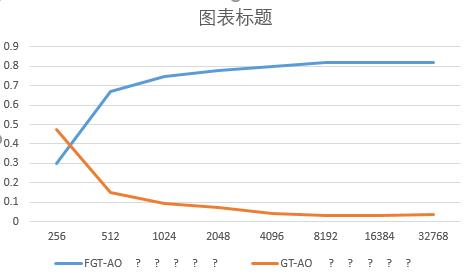
\includegraphics[width=0.4\textwidth]{images/iter.jpg}
\caption{Inflence of Training Iterations}
\end{figure}

\subsection{Related Work}

\subsubsection{Digital Attack v.s. Physical Attack}

In the case of digital attack, the adversary has direct access to the actual data fed into the model. In the case of an attack in the physical world, the adversary does not have direct access to the digital representation of provided to the model. We perform the digital attack in this paper.

In \cite{karmon2018lavan}, we can know, attack can be categorised as image domain attack and network domain attack. For image attack, the new image must at [0,255]. But for the network attack, the value can be any. We do the network domain attack, because we are more interested in investigating the blind-spots of the popular Siamese trackers.

\subsubsection{White Box Attack v.s. Black Box Attack}

In the white box scenario, the adversary has full knowledge of the model including model type, model architecture and values of all parameters and trainable weights.
Traditional adversarial attack methods include FGSM \cite{FGSM} and so on. FGSM means In the black box scenario, the adversary only have limited or no information about the model.

\fi

\end{document}
